\documentclass[a4paper]{article}

\usepackage[english]{babel}
\usepackage[utf8x]{inputenc}
\usepackage{amsmath}
\usepackage{amsfonts}
\usepackage{graphicx}
\usepackage[colorinlistoftodos]{todonotes}

\title{CS 5785 - Applied Machine Learning - Lec.\ 3}
\author{Prof.\ Nathan Kallus, Cornell Tech\\Scribe: TBD}
\date{August 30, 2018}

\begin{document}
\maketitle


\section{Modeling Posterior Probabilities}
Continuing discussion on supervised classification methods.  Recall that when we studied linear regression on the 0/1 model it seemed unnatural; think of the 2D case where we tried to fit a binary output using a linear function (ramp).  Another way of saying this is that we weren't doing a good job of fitting the \emph{posterior probabilities} of t he classes with a linear regression.

\begin{figure}
\centering
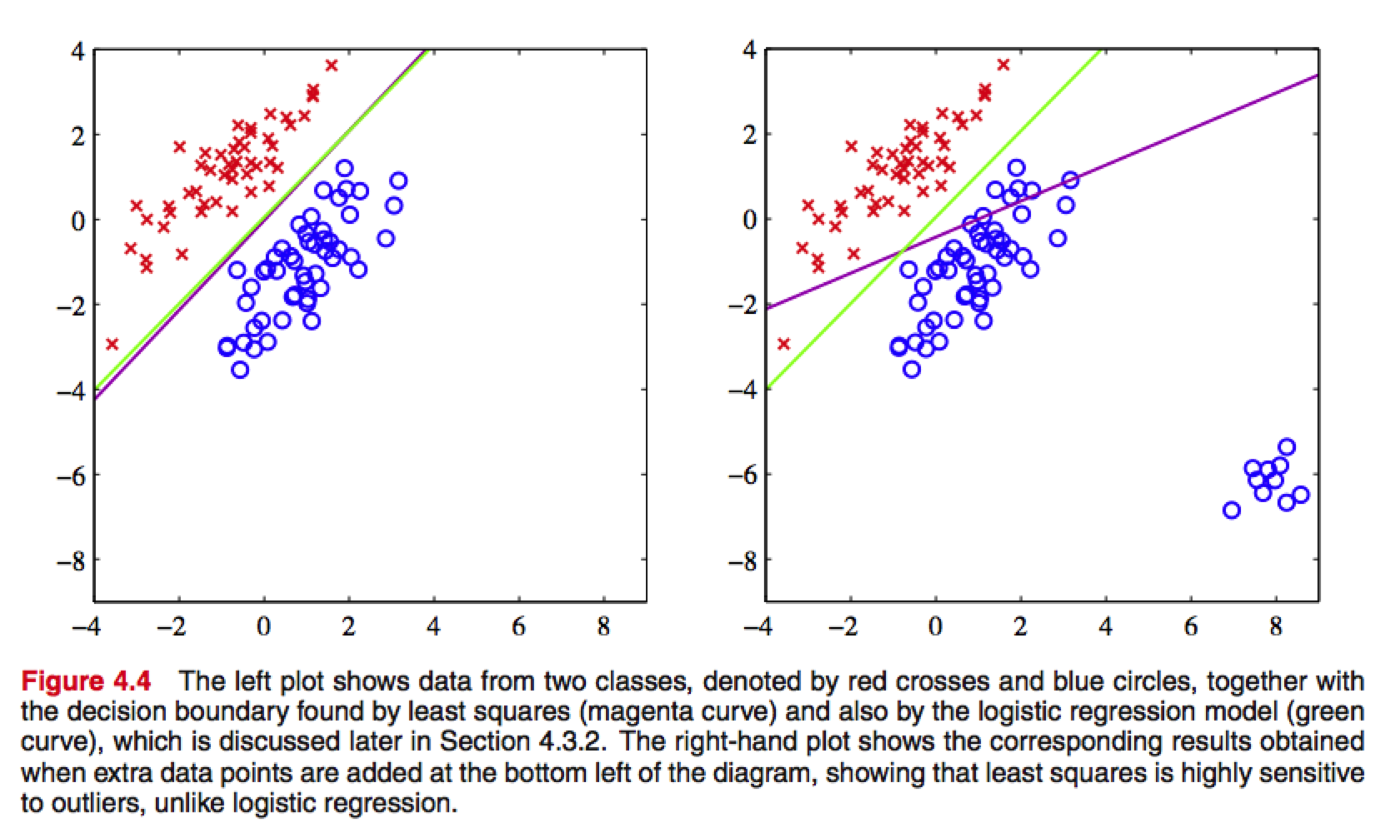
\includegraphics[width=1.0\textwidth]{bishop_fig4_4.png}
\label{fig:faraway}
\end{figure}

In linear regression ({\color{purple}purple}), faraway observations pull on the fit and have ``undue influence'' on the decision boundary; see Figure \ref{fig:faraway}.\footnote{The figure caption refers to the faraway points as outliers; technically for them to be outliers in this case, they'd need to be red. It's better to refer to that clump of blue points simply as ``data far from the margin.''} Such data points  shouldn't matter since they're not anywhere close to the decision boundary. In logistic regression ({\color{green}green}), the decision boundary is minimally affected by these points. Also, with a linear model, we don't get anything resembling a posterior probability that lies within $[0,1]$. Let's look at Bayes' Theorem to see what we can do to fix this. 

\subsection{Bayes' Theorem}
What is the posterior probability (the probability after looking at the evidence)?  The key relationship to remember is
$$\text{Posterior Probability} \propto \text{Prior Probability}\cdot\text{Likelihood}$$
Recall that Bayes' theorem tells us
$$\text{Pr}(\theta|X) = \frac{\text{Pr}(\theta)\text{Pr}(X|\theta)}{\text{Pr}(X)}$$
In this expression: 
\begin{itemize}
\item $\text{Pr}(\theta)$ is the prior probability ("the prior") of the parameter $\theta $ (before looking at evidence).
\item $\text{Pr}(X|\theta)$ is the likelihood or probability of the evidence given the parameters $\theta$.
\item $\text{Pr}(X)$ is the \emph{marginal likelihood}, obtained by summing or integrating out $\theta$. This is the normalization factor.  
\end{itemize}
So far we're not specifying a form (e.g., Gaussian) for $\text{Pr}(\cdot)$ for purposes of generality. $\text{Pr}(X|\theta)$ is easy to collect and $\text{Pr}(\theta|X)$ is what we want. For a spam filter, $X$ would capture features of an email message and $\theta$ would contain parameters that are indicative of good vs.\ spam messages, for example. Finding $\text{Pr}(\theta|X)$ is an inference problem: we infer from some measurements what classes the measurements come from. It is what allows us to create a classifier.

In \emph{logistic regression}\footnote{Despite its name, logistic regression is actually a classification method.} we want the simplicity of a linear model with the feature of ensuring the posterior probabilities remain in the interval $[0,1]$.

\subsection{Log Odds}
A key step in the development of logistic regression is to use the \emph{log odds} or \emph{logit transformation}.  In the binary case ($K=2$) we have two possible classes, $G=1$ and $G=2$, for which the regular (i.e., non-log) odds are given by 
$$\frac{\text{Pr}(G=1|X=x)}{\text{Pr}(G=2|X=x)}$$
Since we only have two possible outcomes, and we know 
$\sum_{l=1}^K \text{Pr}(G=k|X=x)=1$, we have
\begin{equation}
\label{eqn:bernprob}
\text{Pr}(G=2|X=x)=1-\text{Pr}(G=1|X=x)
\end{equation}
We can think of this case as a weighted coin or equivalently a \emph{Bernoulli} random variable.

In logistic regression we assume that the log odds can be expressed as a linear combination of the input features $x\in {\mathbb R}^p$:
$$
\log \frac{\text{Pr}(G=1|X=x)}{\text{Pr}(G=2|X=x)} = \beta_0 + \beta^\top x
$$
Above is an instance of a \emph{generalized linear model}.  Compare this with the ordinary linear model from last lecture in which we assumed we could express the output \emph{itself} as a linear combination of the input features.  If we exponentiate both sides and use Eqn.\ \ref{eqn:bernprob}, we get
\begin{eqnarray}
\label{eqn:prsig}
\text{Pr}(G=1|X=x)&=&\frac{\exp (\beta_0 + \beta^\top x)}{1+\exp(\beta_0 + \beta^\top x)}\\
&=& \frac{1}{1+\exp\left(-(\beta_0 + \beta^\top x)\right)}
\end{eqnarray}

This is a sigmoid function, with the form
$$\sigma(a)=\frac{1}{1+e^{-a}}$$
Sigmoid functions have the desirable property of transitioning smoothly from 0 to 1, like a soft step function, which suits it well for representing posterior probabilities. The sigmoid is also differentiable, which makes it more desirable than step functions. The sigmoid is an example of a \emph{saturating nonlinearity}: going left, the values approach and ultimately go to $0$, and going right, the values similarly approach and ultimately go to $1$.  Via this saturating behavior,  points far away will not impact the decision boundary as much.

\begin{figure}
\centering
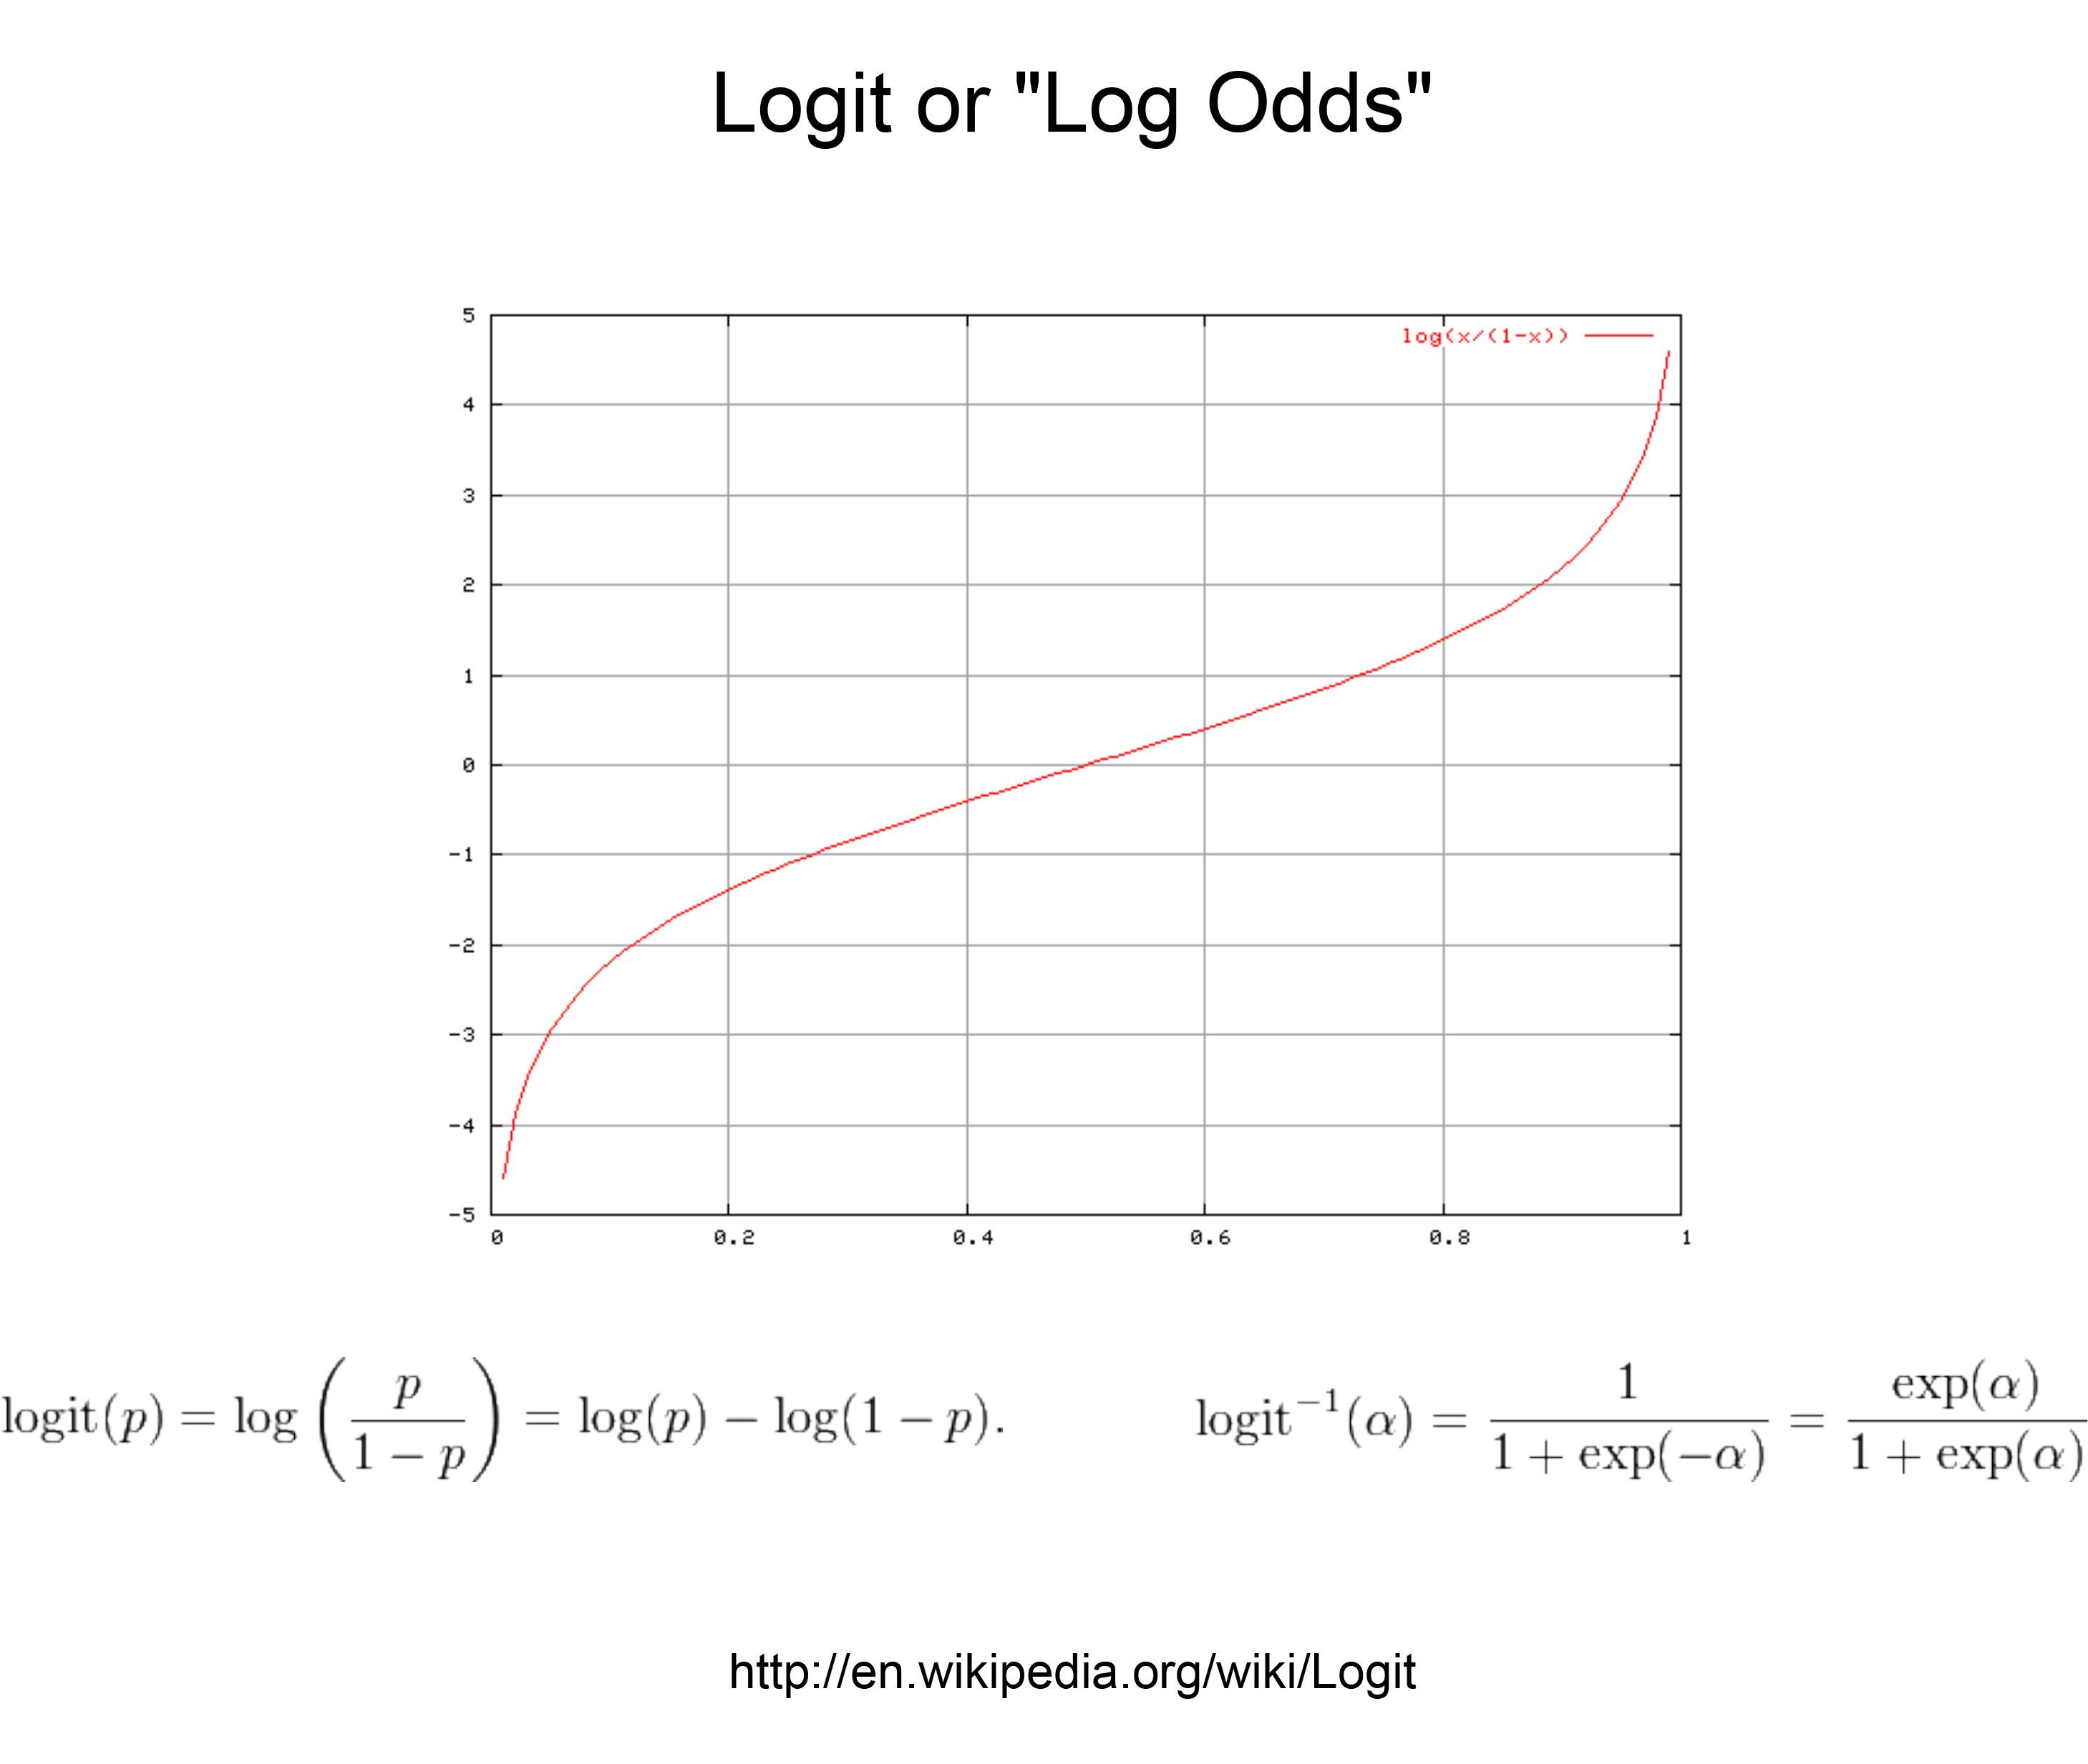
\includegraphics[width=0.75\textwidth]{logit.png}
\end{figure}

\begin{figure}
\centering
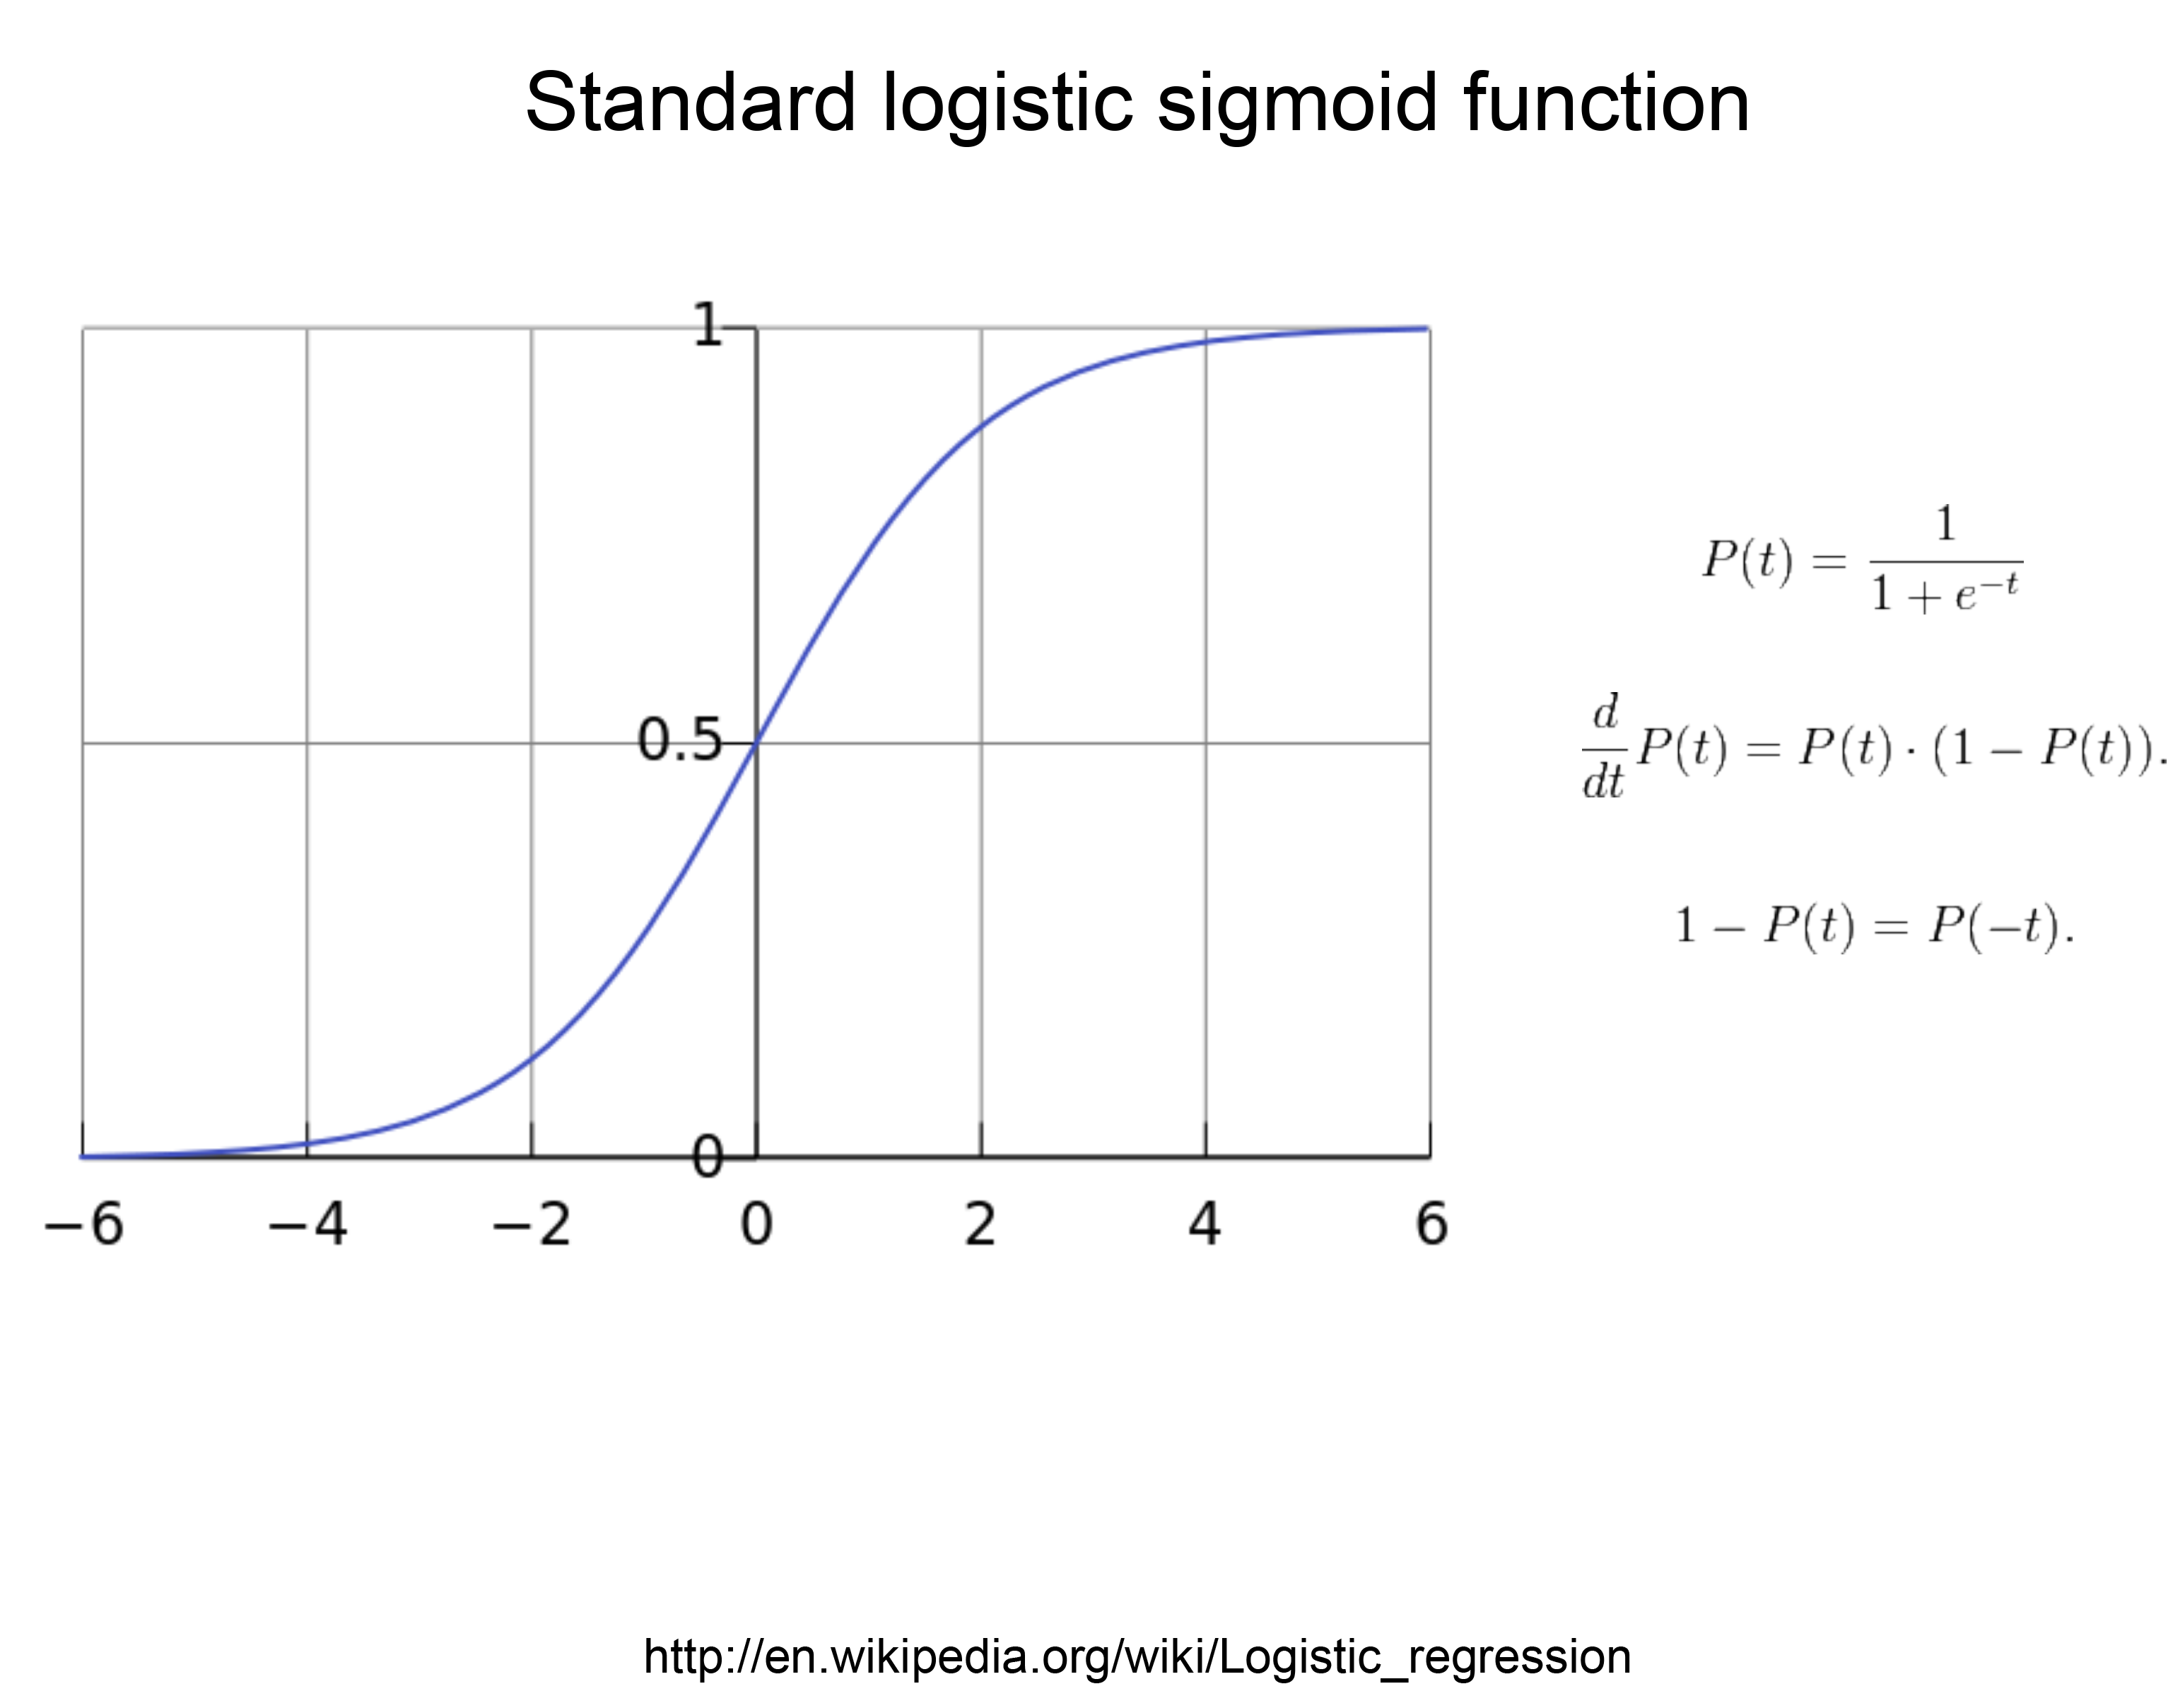
\includegraphics[width=0.75\textwidth]{sigmoid.png}
\end{figure}


\section{Logistic Regression}

Now that we have defined a model for the posterior probabilities, let's see how to fit it. This process is called \emph{logistic regression}.  We'll continue our focus on the 2-class case with the 0/1 response 
$y_i=1$ when $g_i=1$ and 
$y_i=0$ when $g_i=2$.  
To simplify notation, we'll let 
$p_1(x;\theta)=p(x;\theta)$ and 
$p_2(x;\theta)=1-p(x;\theta)$.

There is an old saying that all models are wrong but some models are useful. Logistic model happens to be extremely good at this toy example.

\subsection{Maximum Likelihood Estimation}
We are going to use \emph{maximum likelihood} to fit the model in terms of cost.  Unlike the case for linear regression, we won't have a closed form solution for this.  This will lead us to an instance of an \emph{optimization} method.

The likelihood for $N$ observations is
$$\prod_{i=1}^N p_{g_i}(x_i;\theta)$$
where $p_k(x_i;\theta)=\text{Pr}(G=k|X=x_i;\theta)$, assuming the data is \emph{independent and identically distributed} (iid).  It's preferable, however, to work with the log of the likelihood instead and turn the products into sums:
$$
\ell(\theta) = \sum_{i=1}^N \log p_{g_i}(x_i;\theta)
$$
In the simple 2-class case, using $\beta=\left\{\beta_{0},\beta\right\}$ and tacking on a 1 at the front of $x_i$ to accomodate the intercept, this becomes
$$
\ell(\beta) = \sum_{i=1}^N \left\{ y_i\log p(x_i;\beta) + (1-y_i)\log\left(1-p(x_i;\beta)\right)\right\}
$$
This is in the form of a \emph{cross entropy} function.  The $y_i$ and $1-y_i$ term ``gate'' the two terms in the sum: if $y_i$ is 0 or 1 only one or the other term survives.  If we plug in our expression for $\text{Pr}(G=1|X=x)$ from Eqn.\ \ref{eqn:prsig} we get
$$
\ell(\beta) = \sum_{i=1}^N \left\{ y_i\beta^\top x_i - \log\left(1+e^{\beta^\top x_i}\right) \right\}
$$
This is the quantity we'd like to maximize to fit the model.  And maximizing this means finding the optimal $p+1$ values for $\beta$.

The process of optimization is that you are going to start with some initialization for the  $\beta$. Any given choice of $\beta$, specifies in this case, 2D case, changes the shift and orientation of that sigmoid. So we want a find a $\beta$ that fit the data best. And when we do find that $\beta$, it will maximize this quantity.   

In linear regression, in the 2D case, we fit a linear function (a ramp) and thresholded it to get our decision boundary (a line).  Again visualizing the 2D case, with logistic regression we will obtain our decision boundary by fitting a sigmoid-shaped function to the data (shaped like a soft cliff) and thresholding it at 0.5.  $\beta$ controls the slope and orientation of the sigmoid to separate the two classes.

\begin{figure}
\centering
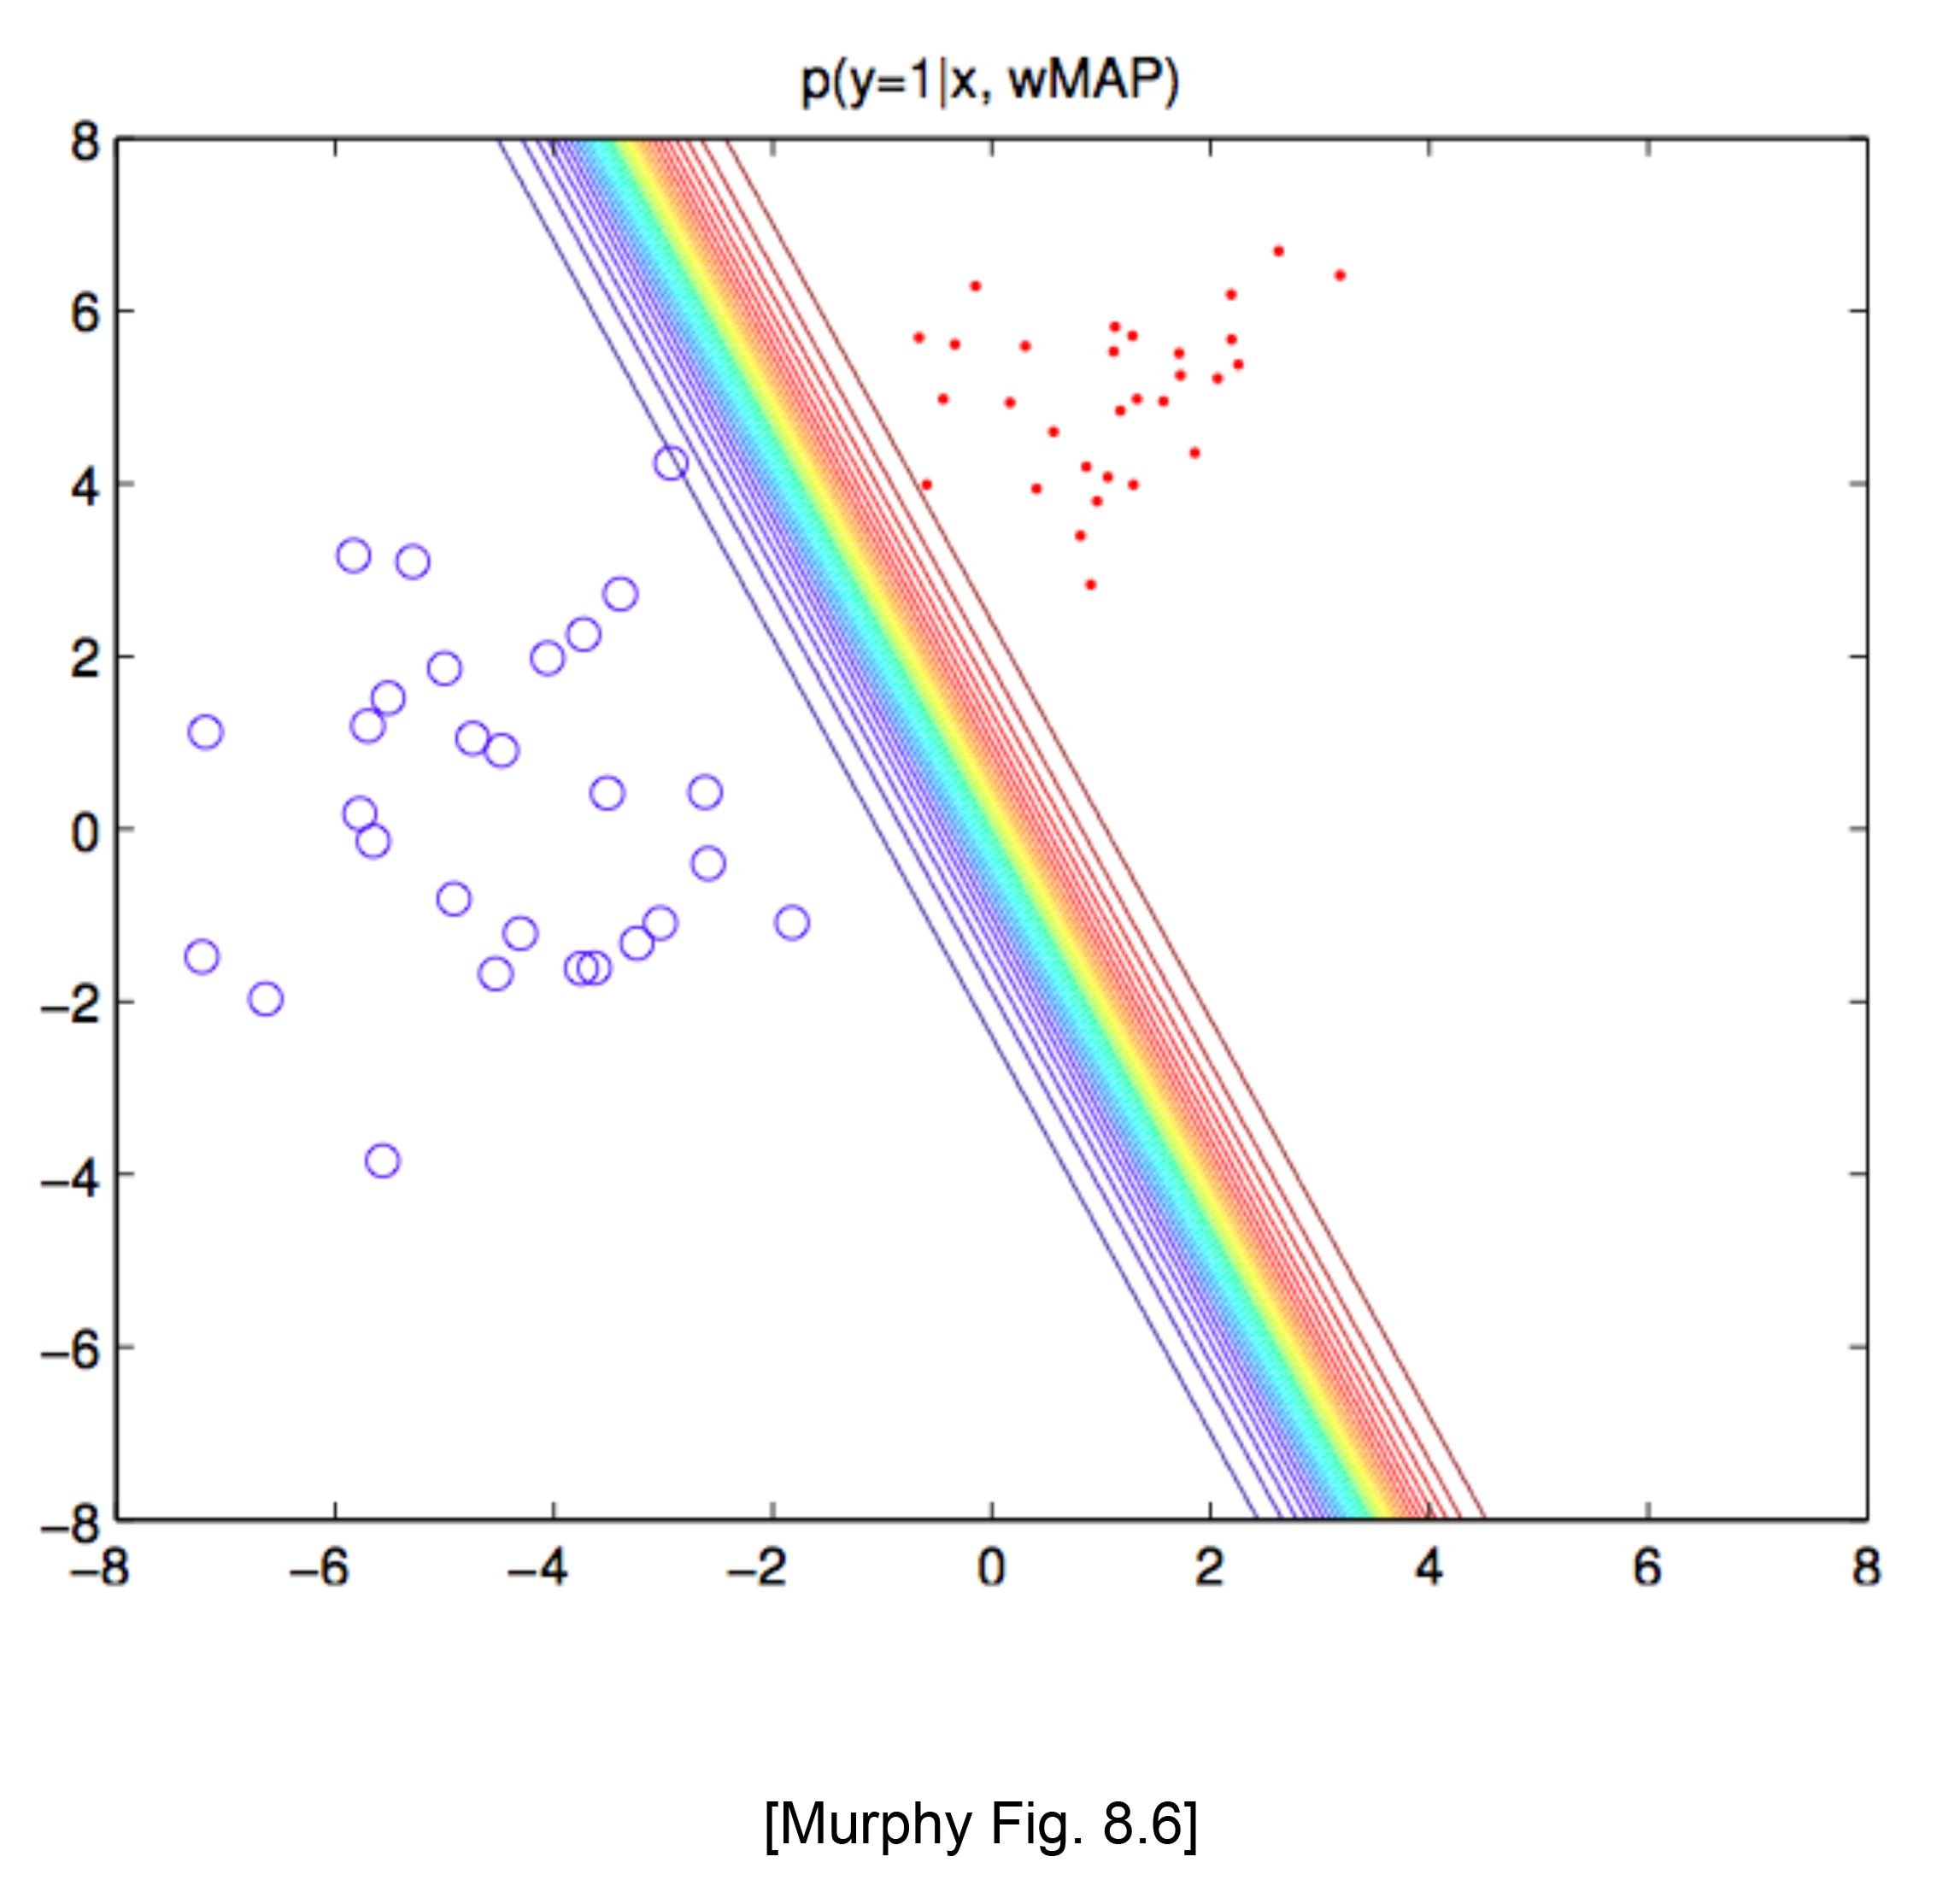
\includegraphics[width=0.75\textwidth]{murphy_fig8_6.png}
\end{figure}

Besides doing a better job of modeling the posterior, the saturating effect of the sigmoid means that data points far from the decision boundary do not have undue influence on the resulting fit.  This is in contrast to linear regression via least squares as we saw earlier in Bishop Fig.\ 4.4.

% say something about the interpretation of the vector of weights fitted using LR

\subsection{Maximizing the Log Likelihood}

To maximize the log likelihood, we set its derivatives with respect to  \ $\beta$ to zero to obtain the \emph{score equations}:
$$
\frac{\partial \ell(\beta)}{\partial \beta} = \sum_{i=1}^N x_i \left(y_i - p(x_i;\beta)\right) = 0
$$
with feature vectors (or data points) $x_i\in\mathbb{R}^{p+1}$, ground truth labels (or \emph{outcome values}) $y_i$ equal to 0 or 1, posterior probabilities $p(x_i;\beta)\in [0,1]$ and a column of $p+1$ zeroes on the RHS.  The gradient represented here is a weighted sum of data points with the weight given by the ground truth label minus the thing we're trying to estimate.  In this respect, the weight is akin to a signed error or discrepancy term.

Recall that the likelihood is just a scalar that is a function of $p+1$ values. You can imagine setting up a high dimensional space for $\beta$ and finding the point with the highest likelihood in this space.  The gradient can tell us in what direction to take a step to increase the likelihood starting from some (possibly random) initialization.

We have $p+1$ equations that are nonlinear in $\beta$. Recall that 
$x_i^1 = 1$ since, by convention, the first entry for any feature vector is $1$. This tells us that 
$$\sum_{i=1}^{N} y_i = \sum_{i=1}^{N} p(x_i;\beta)$$ 
In other words, the expected number of class 1s (the right-hand side) matches the observed number of class 1s (the left-hand side).

To solve the score equations, we will apply the Newton-Raphson algorithm, which uses the second derivative vector counterpart or \emph{Hessian} of the function we wish to optimize; see Murphy Fig. 8.4.  In essence we are finding a 2nd order Taylor series approximation of a function around a given point.  Given this quadratic function, we can solve for the value that maximizes (or minimizes) it in closed form, pick off the next function value at that point and repeat until convergence. When performing the method, we must perform it many times with different random initializations to ensure we do not get stuck in a local extremum. We'll see how to apply Newton-Raphson to our log likelihood function in the next lecture.

\begin{figure}
\centering
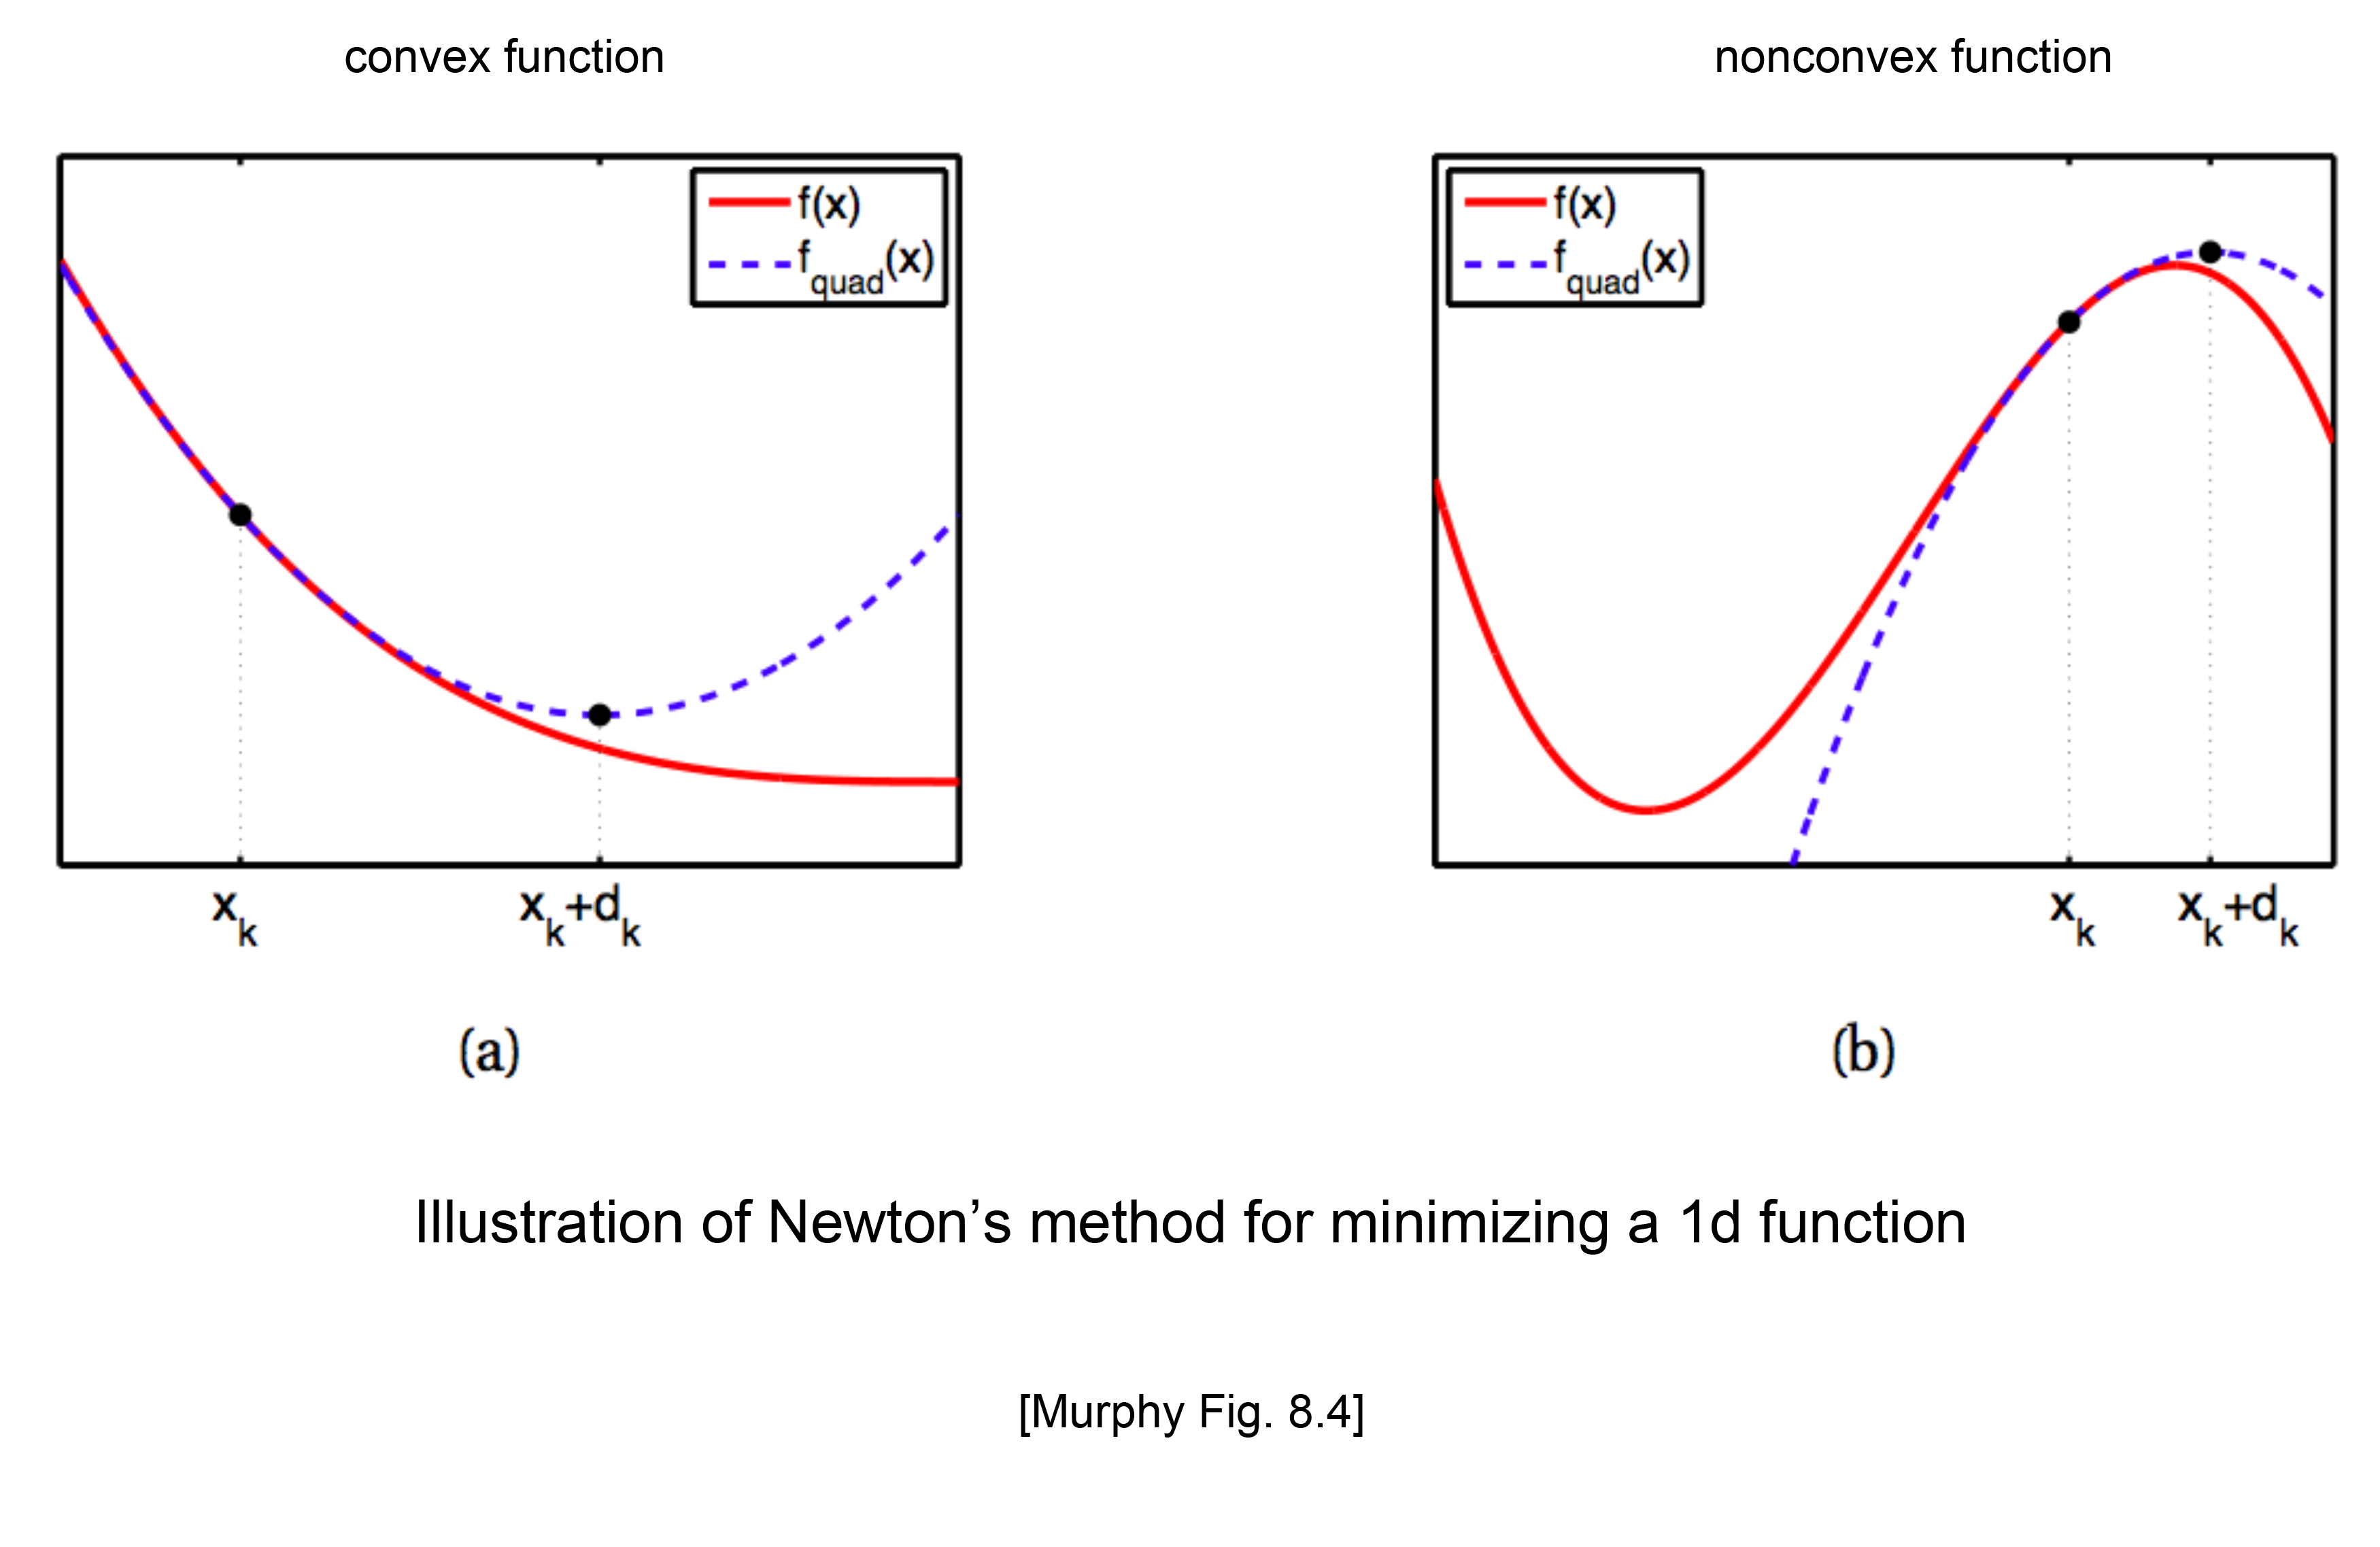
\includegraphics[width=0.75\textwidth]{murphy_fig8_4.png}
\end{figure}

\end{document}
